\documentclass{article}
\usepackage{amsmath}
\usepackage{graphicx}
\usepackage{color}
\usepackage[colorlinks=true, linkcolor=black]{hyperref}
\title{Very Basic Ray Tracer}
\author{Aditya Raj}
\date{March, 2025}

\begin{document}

\maketitle

\tableofcontents

\section{Coordinate System}

In the OCaml standard graphics library, the origin of the drawing window is situated at the bottom left corner. For convenience, we want it in the middle of the window. Thus, we need a wrapper function:

\begin{verbatim}
let plotc x' y' color =
    let x,y = x' + (size_x ()) / 2, y' + (size_y ()) / 2 in 
    set_color (rgb color);
    plot x y;;
\end{verbatim}

This function translates the origin to the middle of the graphics window.

\section{Colors}

We use the additive color model (RGB model), where each color channel is represented by an 8-bit positive integer. Therefore, the range is $[0,255]$. We can treat the triplet of RGB values as a vector. Adding two colors together yields a new color, and multiplying a color by a scalar increases its brightness, i.e.,

$$k (r, g, b) = (kr, kg, kb)$$

There is a chance that any channel value may go out of the range $[0,255]$ while manipulating colors. We can handle this as follows:

Suppose there is a channel value $x$:
\begin{itemize}
    \item If $x > 255$, then we set $x = 255$.
    \item If $x < 0$, then we set $x = 0$.
\end{itemize}

This process is called \textbf{clamping}.

\section{Scene}

The scene is simply a set of objects that we want to render on the screen.

To represent objects in a scene, we need to use a 3D coordinate system that employs real numbers to represent continuous values, which are then mapped to a discrete 2D graphics window while drawing.

\begin{figure}[h]
    \centering
    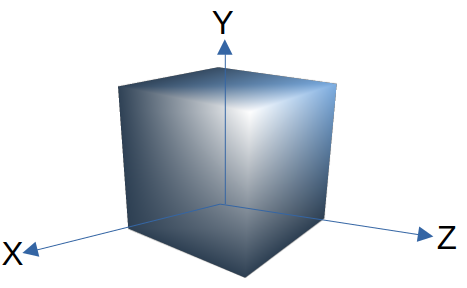
\includegraphics[width=0.5\textwidth]{./figs/3Dcoodinate.png}
    \caption{3D Coordinate System}
\end{figure}

It is clear from the figure which axes point in which direction.

The viewing position from which we look at the scene is called the \textbf{camera position}. We assume that the camera is fixed and occupies a single point in space, which will often be the origin $O(0,0,0)$.

The \textbf{camera orientation} is the direction in which the camera points, or from where rays enter the camera. We will assume the camera orientation to be $Z_+$, the positive z-axis.

The frame has dimensions $V_w$ and $V_h$ and is frontal to the camera (perpendicular to the camera orientation, irrespective of camera position, in our case perpendicular to $Z_+$) and at a distance $d$ away from the camera. Technically, this is called the \textbf{viewport}.

The angle visible from the camera is called the \textbf{field of view} (FOV). It depends on the distance $d$ from the camera to the viewport and the dimensions of the viewport $V_w$ and $V_h$.

In our case, we assume 

$$V_w = V_h = d = 1 \implies FOV \approx 53^\circ$$

We will represent the coordinates of the viewport as $(V_x,V_y)$ in worldly units and the graphics window as $(G_x,G_y)$ in pixels. Thus, the conversion is given by:

$$V_x = G_x \times \frac{V_w}{G_w}$$

$$V_y = G_y \times \frac{V_h}{G_h}$$

where $G_w$ and $G_h$ are the maximum width and height of the graphics window, respectively.

\begin{verbatim}
let g_to_viewport gx gy =
    let vw = 1. in (* setting width and height of viewport *)
    let vh = 1. in
    let vx = (float gx) .* vw /. float (size_x ()) in 
    let vy = (float gy) .* vh /. float (size_y ()) in 
    let d = 1 in (* z coordinate of viewport *)
    vx, vy, d;;
\end{verbatim}

However, we know that the viewport is in 3D space, so it also has $V_z = d$ for every point on this viewport (in mathematical terms, called the \textit{projection plane}). \\
Thus, for every pixel $(G_x, G_y)$ on the graphics window, we can calculate the corresponding $(V_x, V_y, V_z)$ of the viewport.

\section{Rays}

The rays are simply straight lines emanating from the origin $O$ and passing through various points of the viewport, ultimately intersecting the objects in the scene.

We will represent a straight line using the parametric form:

$$P = O + t(V - O)$$

Here:
\begin{itemize}
    \item $P$ is any point on the line.
    \item $O$ is the origin (where the camera is positioned).
    \item $V$ is any point on the viewport.
    \item $t$ is the parameter, where $-\infty < t < \infty$.
\end{itemize}

We vary $t$ to obtain various points on the straight line.

Also note that:
\begin{itemize}
    \item If $t < 0$, then $P$ is behind the camera.
    \item If $0 \leq t \leq 1$, then $P$ lies between the camera and the viewport.
    \item If $t > 1$, then $P$ is in front of the viewport.
\end{itemize}

\section{Sphere}

The sphere is the simplest geometric object and will be used as an object in the scene.

We represent a sphere as:

$$\langle P - C, P - C \rangle = r^2$$

Here:
\begin{itemize}
    \item $P$ is a point on the surface of the sphere.
    \item $C$ is the center of the sphere.
    \item $r$ is the radius of the sphere.
\end{itemize}

\section{Rays Intersecting Objects in the Scene}

Currently, we only have a sphere.

\subsection{Intersection of Straight Line and Sphere}

Let $P$ be the point of intersection; it is a common point to both the ray and the sphere.

The equation of the ray is:

$$P = O + t \vec{D}$$

where $\vec{D} = V - O$ is the direction of the ray.

The equation of the sphere is:

$$\langle P - C, P - C \rangle = r^2$$

Substituting the value of $P$ into the equation of the sphere gives:

$$\langle O + t \vec{D} - C, O + t \vec{D} - C \rangle = r^2$$

$$\langle t \vec{D} + \vec{CO}, t \vec{D} + \vec{CO} \rangle = r^2$$

$$\langle t \vec{D} + \vec{CO}, t \vec{D} \rangle + \langle t \vec{D} + \vec{CO}, \vec{CO} \rangle = r^2$$

$$\langle t \vec{D}, t \vec{D} \rangle + \langle t \vec{D}, \vec{CO} \rangle + \langle \vec{CO}, t \vec{D} \rangle + \langle \vec{CO}, \vec{CO} \rangle = r^2$$

Finally, we arrive at the quadratic equation:

$$at^2 + bt + c = 0$$

where:
\begin{itemize}
    \item $a = \| \vec{D} \|^2$
    \item $b = 2 \langle \vec{D}, \vec{CO} \rangle$
    \item $c = \| \vec{CO} \|^2 - r^2$
\end{itemize}

This makes sense because a ray can intersect a sphere at either 0, 1, or 2 points.

We can now find the values of $t$ using the quadratic formula:

$$t_{1,2} = \frac{-b \pm \sqrt{b^2 - 4ac}}{2a}$$

After finding the values of $t$, we can substitute them back into the equation of the ray to find the point $P$. We should be careful to take the closest point $P$ (the one which is visible to the camera) for which $t > 1$ (indicating that the objects are in front of the viewport).

\section{Lighting}

We use white light and assume that light has the same intensity irrespective of the distance from the source.

\subsection{Point Lights}

Point lights can be completely described by:
\begin{itemize}
    \item The coordinate $Q$ of their location.
    \item The intensity of light.
\end{itemize}

Any vector from an arbitrary point $P$ to the light source $Q$ will be denoted by $\vec{L}$.

\subsection{Directional Lights}

Directional lights are used to represent light sources that are situated very far away compared to the distances between objects in the scene. Thus, rays of light coming from these sources are essentially parallel to each other. Therefore, $\vec{L}$ is the same for every point $P$ in the scene.

To model these lights, we need:
\begin{itemize}
    \item A direction vector $\vec{L}$.
    \item The intensity of light.
\end{itemize}

\subsection{Ambient Light}

In real life, an object that does not receive direct light is not completely dark because reflected light illuminates it. To avoid treating every object as a light source, we will use ambient light, which essentially illuminates every object in the scene.

To model ambient light, we need:
\begin{itemize}
    \item The intensity of light.
\end{itemize}

\subsection{Lighting a Point}

We define a type for light as follows:

\begin{verbatim}
(* type for light *)
(* kind of light is represented by k field - *)
(* p - for point source *)
(* d - for directional light *)
(* a - for ambient source *)
type light = 
  {
    k : char;
    i : float;
    v : point option
  }
\end{verbatim}

The field $v$ stores:
\begin{itemize}
    \item The location of the point, in the case of a point source.
    \item The direction vector, in the case of a directional light.
    \item `None`, in the case of an ambient source.
\end{itemize}

The sum of all intensities of light should equal 1. If it does not, some points in the scene will be overexposed.

\subsection{Diffuse Reflection}

Now we calculate how much a point should be illuminated by a point source and a directional source through diffuse reflection.

Consider a point $P$ in the scene. Let $\vec{N}$ be a normal vector at $P$, and $\vec{L}$ be the directional vector. In the case of directional light, we are already given $\vec{L}$. However, in the case of a point light source, we need to compute it from the position of the light source and the coordinates of point $P$. Let $l$ denote the width of the light (proportional to intensity) and $x$ denote the length over which light spreads. Let $RS$ be perpendicular to $\vec{L}$, and $Q$ be the point of intersection.

The ratio $\frac{l}{x}$ represents the drop in intensity after reflection. For example, if light is perpendicular to point $P$ on the surface, $\frac{l}{x} = 1$.

\begin{figure}[h]
    \centering
    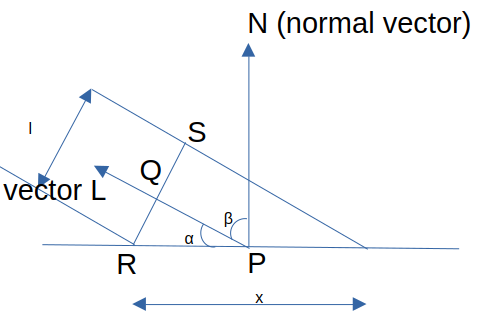
\includegraphics[width=0.5\textwidth]{./figs/intensity.png}
    \caption{Intensity After Reflection}
\end{figure}

Consider triangle $PQR$, which is a right-angled triangle. It is easy to see that:

$$\angle PRQ = \beta$$

Now,

$$\cos \beta = \frac{l/2}{x/2} = \frac{l}{x}$$

We know that:

$$\langle \vec{L}, \vec{N} \rangle = \|\vec{L}\| \|\vec{N}\| \cos \beta$$

Thus,

$$\cos \beta = \frac{\langle \vec{L}, \vec{N} \rangle}{\|\vec{L}\| \|\vec{N}\|}$$

If $\beta > 90^\circ$, then the point is illuminated from the back side of the surface. In that case, we treat it as zero.

We will multiply the intensity of light by this factor $\cos \beta$ to get the intensity after reflection.

A single point in a scene is illuminated by many sources, which may be of different kinds. We simply add all the light intensities that hit the point and finally multiply the total intensity by the color of the point. This essentially increases or decreases the brightness.

Mathematically, we express this as:

\[I_{\text{diffused}} = \sum I_i \frac{\langle \vec{L_i}, \vec{N} \rangle}{\|\vec{L}_i\| \|\vec{N}\|}\]


where:
\begin{itemize}
    \item $I_{\text{diffused}}$ is the intensity due to diffuse reflection.
    \item $I_i$ is the intensity of the $i^{th}$ light source, which can be a point source or a directional light.
    \item $\vec{L_i}$ is the directional vector of the $i^{th}$ light.
\end{itemize}

\subsection{Specular Reflection}

To model specular reflection, we use the fact that the angle made by the incident ray with the normal is equal to the angle made by the reflected ray with the normal.

\begin{figure}[h]
    \centering
    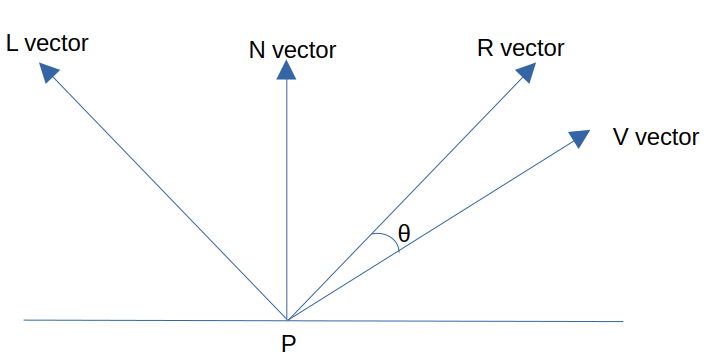
\includegraphics[width=0.5\textwidth]{./figs/intensityspecular.png}
    \caption{Intensity of Specular Reflection}
\end{figure}

Here:
\begin{itemize}
    \item $\vec{L}$ is the directional vector of light pointing from $P$ to the source or from point $P$ on the surface to the point source light.
    \item $\vec{R}$ is the reflected light, which makes the same angle with $\vec{N}$ as $\vec{L}$.
    \item $\vec{V}$ is the view vector from point $P$ on the surface to the camera.
    \item $\vec{N}$ is the normal vector.
\end{itemize}

First, we express $\vec{R}$ in terms of $\vec{L}$ and $\vec{N}$.

We know that $\vec{L}$ can be split into two vectors: one parallel to $\vec{N}$ and another perpendicular to it.

$$\vec{L_{\| N}} = \langle \vec{L}, \hat{N} \rangle \hat{N}$$

Since 

$$\vec{L_{\| N}} + \vec{L_{\perp N}} = \vec{L}$$

we have:

$$\vec{L_{\perp N}} = \vec{L} - \langle \vec{L}, \hat{N} \rangle \hat{N}$$

Thus,

$$\vec{R} = \vec{L_{\| N}} - \vec{L_{\perp N}}$$

This simplifies to:

$$\vec{R} = 2 \langle \vec{L}, \hat{N} \rangle \hat{N} - \vec{L}$$

Now we determine the intensity due to specular reflection. For $\theta = 0$, the reflected vector and view vector align, resulting in maximum brightness. If $\theta = 90^\circ$, no component of the reflected ray is in the direction of the view vector, so brightness is zero in this case.

For $0 \leq \theta \leq 90^\circ$, we use $\cos \theta$ to model brightness. We define $s$ to vary the shininess of different objects.

The final expression for brightness due to specular reflection is:

$$I_{\text{specular}} = \sum I_i (\cos \theta)^s = \sum I_i \left( \frac{\langle \vec{R_i}, \vec{V_i} \rangle}{\|\vec{R_i}\| \|\vec{V_i}\|} \right)^s$$

Note that if $\theta > 90^\circ$, we might get a negative total intensity, which doesn't make sense. In those cases, we set the term to zero as before.

Combining both diffuse and specular brightness, along with ambient light, we get:

$$I_{\text{total}} = I_a + \sum I_i \left[ \frac{\langle \vec{L_i}, \vec{N} \rangle}{\|\vec{L}_i\| \|\vec{N}\|} + \left( \frac{\langle \vec{R_i}, \vec{V} \rangle}{\|\vec{R_i}\| \|\vec{V}\|} \right)^s \right]$$

where:
\begin{itemize}
    \item $I_{\text{total}}$ is the total intensity at the point.
    \item $I_a$ is the intensity of ambient light.
    \item $I_i$ is the intensity of the $i^{th}$ light, which could be a point source or directional light.
    \item $\vec{L_i}$ is the incident vector of the $i^{th}$ light.
    \item $\vec{R_i}$ is the reflected vector of the $i^{th}$ light.
    \item $\vec{N}$ is the normal vector at a point.
    \item $\vec{V}$ is the view vector at a point.
\end{itemize}

\subsection{Casting Shadows at a Point}

A shadow is the obstruction of light by one or more objects at a point. 

What this means for us is that we need to check if a particular light, such as a point source or directional light, has a ray that intersects any other object in the scene before reaching the point for which we are calculating illumination due to that light. If that intersection occurs, then we do not include that light's intensity in the calculation of the total intensity; otherwise, we do.

To do this, we shoot a ray from the point of interest (for which we want to know whether it is shadowed) in the direction of the light source.

This ray is represented as:

$$P + t \vec{L}$$

Here:
\begin{itemize}
    \item $P$ is the point of interest.
    \item $\vec{L}$ is the ray of light from $P$ toward the light source.
    \item $t$ is the parameter. For a point source, $t \in [0^+, 1]$ (at $t=1$, we reach the light source itself), and for directional light, $t \in [0^+, \infty]$. We know that a point on a sphere will definitely intersect itself, so practically we take $0.0001$ instead of $0^+$.
\end{itemize}

Next, we find the closest intersection of the sphere with the ray in the suitable range. If a sphere exists, then only ambient light illuminates that point; otherwise, specular and diffuse reflections also occur.

\subsection{Mirror Reflection at a Point}

After a ray from a camera intersects at a point on an object, we find the reflected ray at that point (along with its color) and then again shoot a reflected ray to find out if it intersects another object and calculate the color. We can do this as many times as we like (but usually after 3 iterations, we get diminishing returns per computation) and eventually take a weighted sum of all the colors utilizing the reflection property of spheres.

\section{Rendering}

We iterate over every pixel of the graphics window and find the corresponding point on the viewport, then shoot out a ray from the camera through that point on the viewport. If that ray intersects an object in the scene, we calculate the color and set that pixel to that color.

\begin{verbatim}
let o = (0,0,0);; (* the origin O *)
let gw, gh = size_x (), size_y () in (* max width and height of graphics window *)
for x = -gw/2 to gw/2 do 
    for y = -gh/2 to gh/2 do 
        let v = g_to_viewport x y in
        let d = sub3 v o in
        let color = rtx o d 1. infinity ls ll in 
        plotc x y color
    done;
done;;
\end{verbatim}
\end{document}